% 限制性三体问题
% 二体系统|平面圆形轨道|限制性三体问题

\pentry{中心力场问题\upref{CenFrc},开普勒问题\upref{CelBd}}

在中心力场问题中,只需把质点质量 $m$ 和位矢 $\vec r$ 分别替换成约化质量 $\mu M$ 和相对矢量 $\vec R$ 即可将单质点中心力场问题的规律拓展到二体系统.

在\autoref{TriLim_fig1}  所示的惯性坐标系 $XOY$ 中,天体A和天体B距离为 $R$ ,质量分别为 $M_1$ 和 $M_2$,总质量为 $M$,原点$0$为该二体系统的质心.记 $M_1=\mu M$,则 $M_2=(1-\mu)M$.由开普勒问题中的结论,可以推知,天体A和天体B的运动轨迹是坐标平面中两条相似的圆锥曲线.
\begin{figure}[ht]
\centering
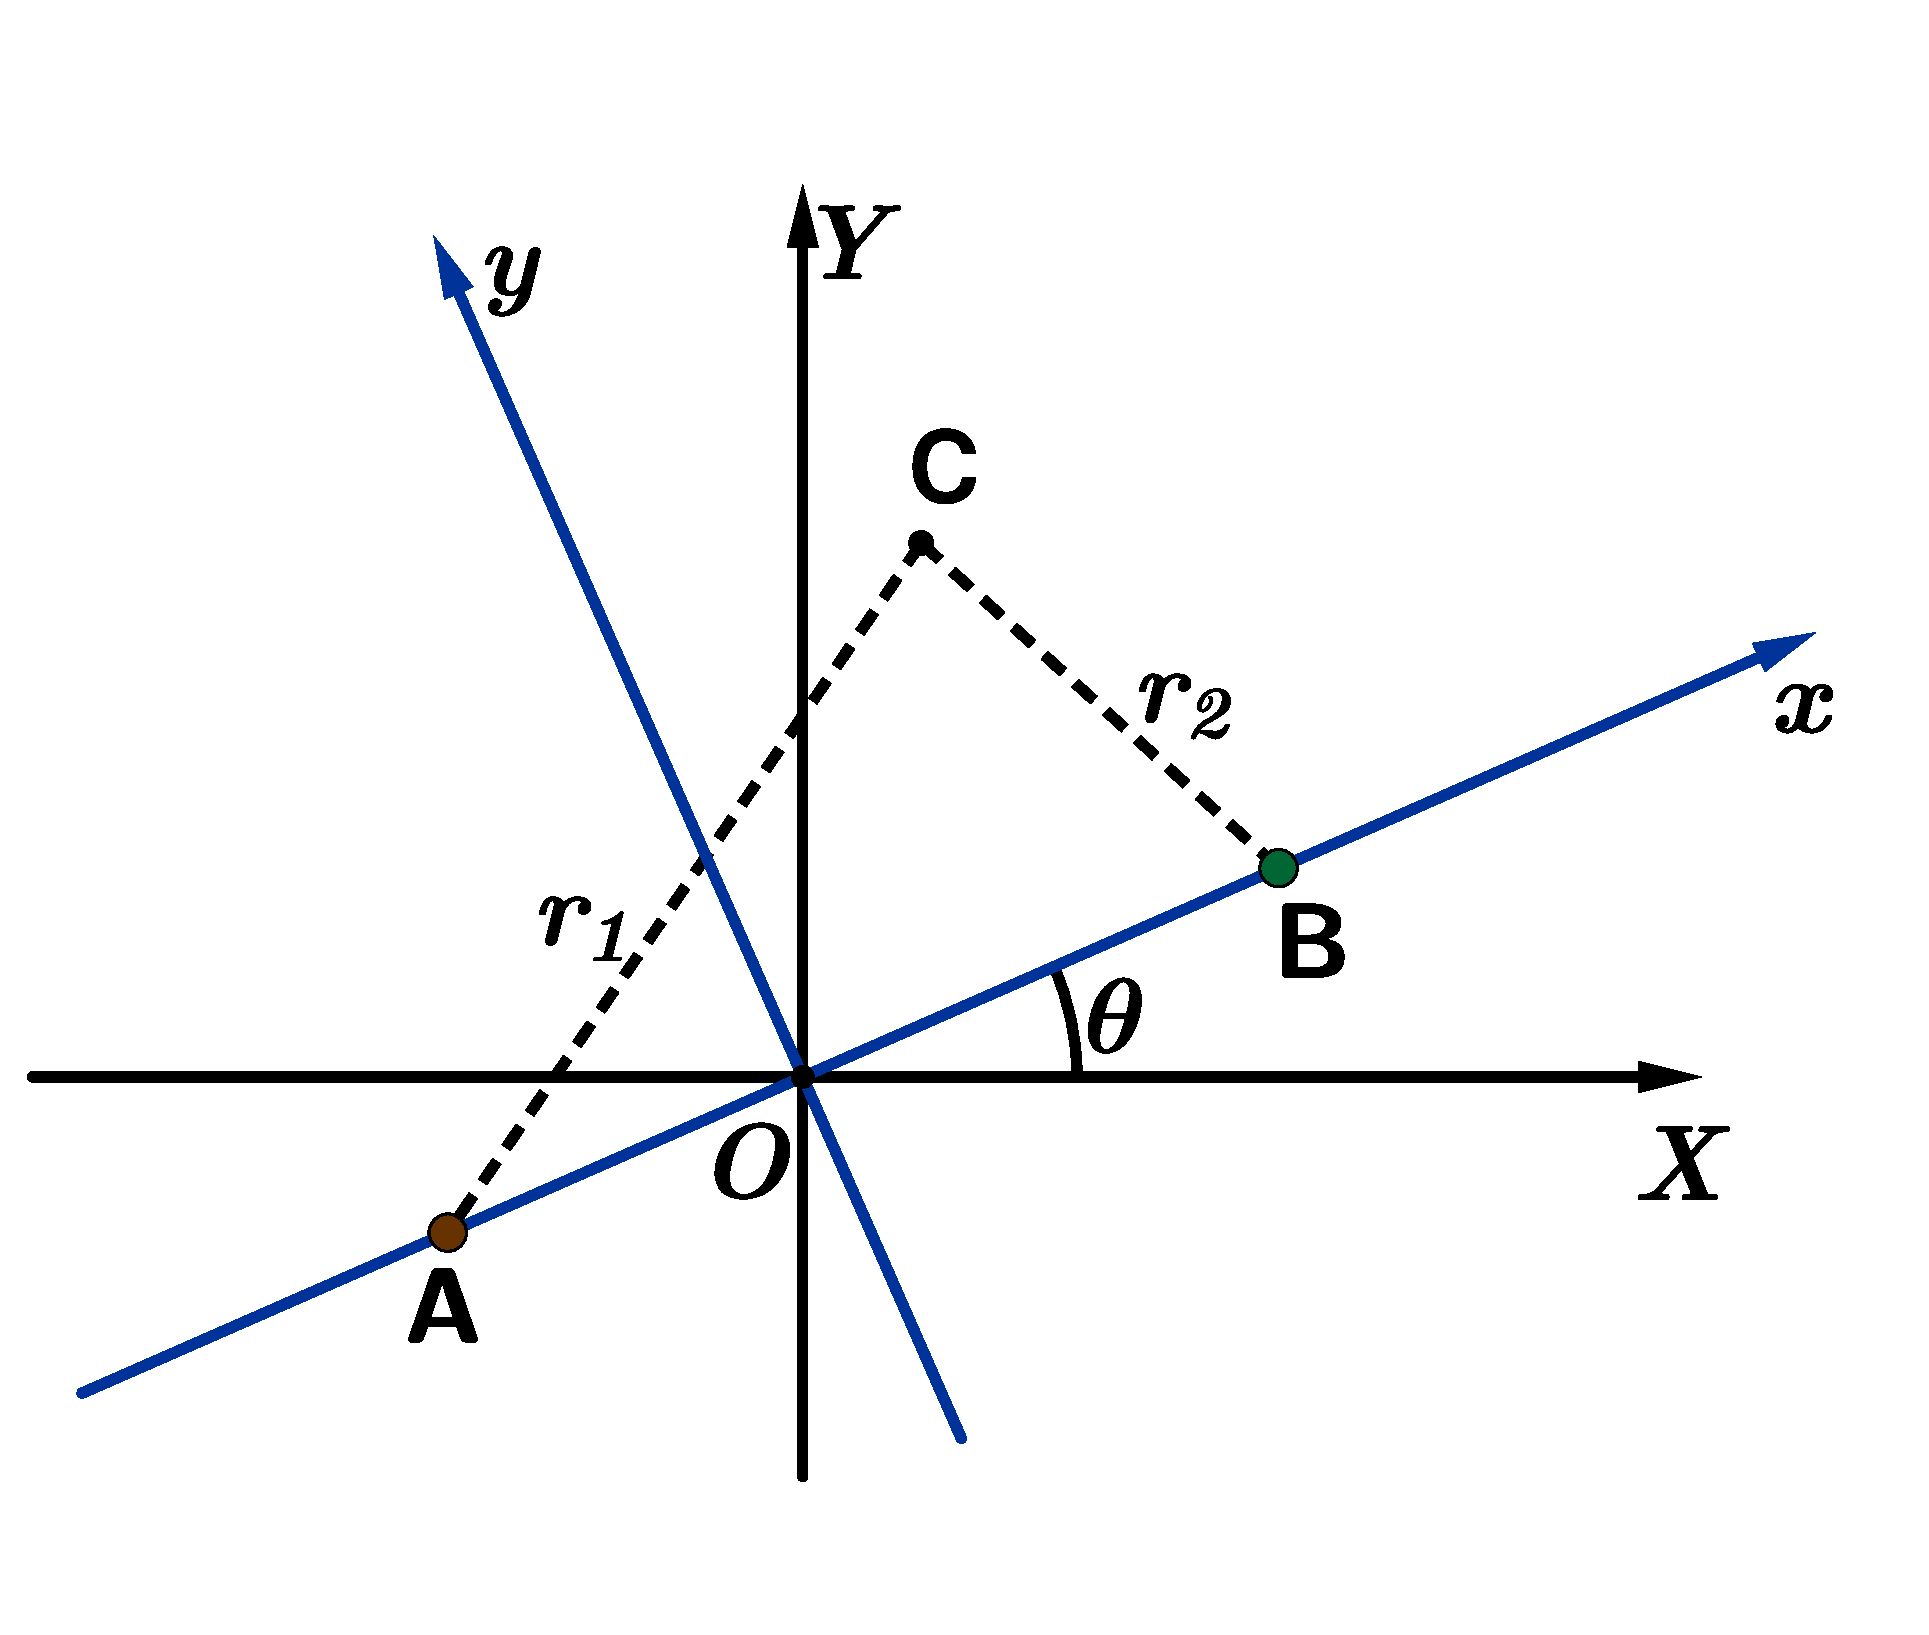
\includegraphics[width=8cm]{./figures/TriLim1.pdf}
\caption{限制性三体问题} \label{TriLim_fig1}
\end{figure}

在\autoref{TriLim_fig1}  的二体系统中再添加一个质点,其质量 $m$ 足够小,以至于该质点对原二体系统的影响可以忽略不计.在此条件下该系统的运动问题,称为\bb{限制性三体问题}.

假设当前时刻,A、B连线相对惯性坐标系的角速度为 $\omega$,与 $X$ 轴正方向夹角为 $\theta$.以A、B连线为 $x$ 轴建立旋转坐标系 $xOy$.记质点C在旋转系中的坐标为 $(x,y,z)$,在惯性系中的位置矢量为 $\vec r$,两者有如下关系
\begin{equation}%1
\vec r=
\begin{pmatrix}
\cos\theta &-\sin\theta &0 \\
\sin\theta &\cos\theta  &0 \\
0               &0                 &1  \\
\end{pmatrix} 
\pmat{x\\ y\\ z }
\end{equation}

将上式关于时间求导,可得
\begin{equation}%2
\dot{\vec r}=\pmat{\qty(\dot{x}-\omega y)\cos\theta -\qty(\omega x+\dot{y})\sin\theta \\ \qty(\dot{x}-\omega y)\sin\theta -\qty(\omega x+\dot{y})\cos\theta \\ \dot{z} }
\end{equation}
于是,可求出质点的动能
\begin{equation}\label{TriLim_eq3}%3
T=\frac{1}{2}m|\dot{\vec r}|^2=\frac{1}{2}m\qty[\qty(\dot{x}-\omega y)^2+\qty(\omega x+\dot{y})^2+\dot{z}^2]
\end{equation}

记质点C与天体A、B的距离分别为 $r_1$ 和 $r_2$,则质点C的引力势能可表达为
\begin{equation}\label{TriLim_eq4}%4
\begin{aligned}
U&=-\frac{\mu GMm}{r_1}-\frac{(1-\mu)GMm}{r_2}\\
 &=-\frac{\mu GMm}{\sqrt{[x+(1-\mu)R]^2+y^2+z^2}}-\frac{(1-\mu)GMm}{\sqrt{(x-\mu R)^2+y^2+z^2}}
\end{aligned}
\end{equation}

在惯性系中,质点C对坐标原点的角动量为
\begin{equation}%5
\vec L=m\vec r \times \dot{\vec r}
\end{equation}
这里只考虑角动量在 $Z$ 轴方向上的分量
\begin{equation}\label{TriLim_eq6}%6
\begin{aligned}
L_z &= m 
\vmat{
x\cos\theta-y\sin\theta &{x\sin\theta+y\cos\theta}\\
\qty(\dot{x}-\omega y)\cos\theta -\qty(\omega x+\dot{y})\sin\theta &{\qty(\dot{x}-\omega y)\sin\theta -\qty(\omega x+\dot{y})\cos\theta }
}\\
&=m\qty[\omega \qty(x^2+y^2)+x\dot{y}-\dot{x}y]
\end{aligned}
\end{equation}

在没有外力或外力矩的情况下,三体系统的总角动量和总机械能守恒.由于先前假设质点C的引入不影响原二体系统的运动,因此在限制性三体问题中,天体A和天体B的机械能及角动量依旧守恒,于是质点C的机械能和角动量也守恒.

以上的讨论中,并不限制天体A和天体B的距离 $R$ 和角速度 $\omega$ 在运动过程中为定值,换句话说,无论原二体系统的运动模式是何种圆锥曲线,以上的讨论都成立.
